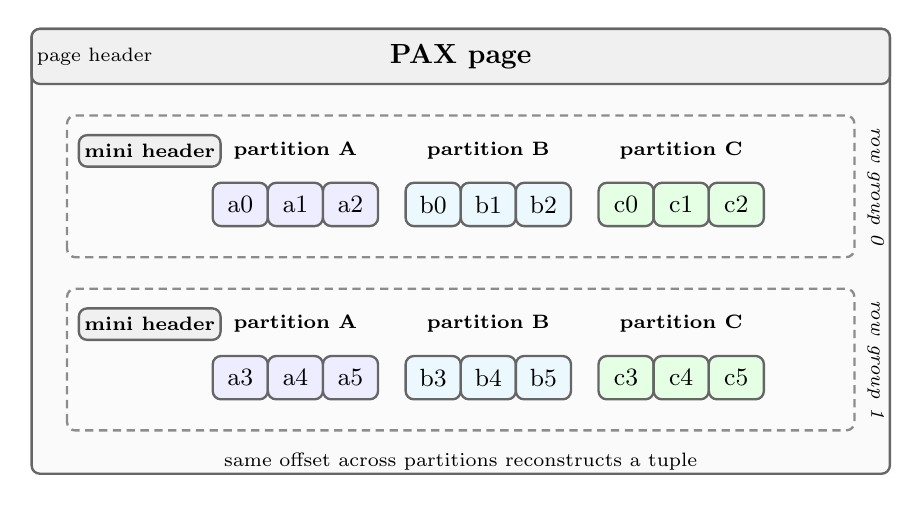
\begin{tikzpicture}[
    x=1cm,y=1cm,
    every node/.style={font=\small},
    frame/.style={draw=black!60, rounded corners=3pt, line width=0.85pt},
    header/.style={frame, fill=gray!12},
    group/.style={draw=black!45, rounded corners=3pt, line width=0.85pt, densely dashed, fill=gray!3},
    acell/.style={frame, minimum width=0.70cm, minimum height=0.55cm, fill=blue!7},
    bcell/.style={frame, minimum width=0.70cm, minimum height=0.55cm, fill=cyan!8},
    ccell/.style={frame, minimum width=0.70cm, minimum height=0.55cm, fill=green!10}
]
    \draw[frame, fill=gray!4] (0,0) rectangle (10.9,5.65);
    \draw[header] (0,4.95) rectangle (10.9,5.65);
    \node[font=\bfseries] at (5.45,5.30) {PAX page};
    \node[font=\scriptsize] at (0.80,5.30) {page header};

    \draw[group] (0.45,2.75) rectangle (10.45,4.55);
    \draw[group] (0.45,0.55) rectangle (10.45,2.35);

    \draw[header] (0.60,3.90) rectangle (2.40,4.30);
    \draw[header] (0.60,1.70) rectangle (2.40,2.10);
    \node[font=\bfseries] at (1.50,4.10) {\scriptsize mini header};
    \node[font=\bfseries] at (1.50,1.90) {\scriptsize mini header};

    \foreach \x/\lbl in {3.35/A,5.80/B,8.25/C} {
        \node[font=\scriptsize\bfseries] at (\x,4.10) {partition \lbl};
        \node[font=\scriptsize\bfseries] at (\x,1.90) {partition \lbl};
    }

    \node[acell] at (2.65,3.42) {a0};
    \node[acell] at (3.35,3.42) {a1};
    \node[acell] at (4.05,3.42) {a2};
    \node[bcell] at (5.10,3.42) {b0};
    \node[bcell] at (5.80,3.42) {b1};
    \node[bcell] at (6.50,3.42) {b2};
    \node[ccell] at (7.55,3.42) {c0};
    \node[ccell] at (8.25,3.42) {c1};
    \node[ccell] at (8.95,3.42) {c2};

    \node[acell] at (2.65,1.22) {a3};
    \node[acell] at (3.35,1.22) {a4};
    \node[acell] at (4.05,1.22) {a5};
    \node[bcell] at (5.10,1.22) {b3};
    \node[bcell] at (5.80,1.22) {b4};
    \node[bcell] at (6.50,1.22) {b5};
    \node[ccell] at (7.55,1.22) {c3};
    \node[ccell] at (8.25,1.22) {c4};
    \node[ccell] at (8.95,1.22) {c5};

    \node[font=\scriptsize\itshape, rotate=-90] at (10.72,3.65) {row group 0};
    \node[font=\scriptsize\itshape, rotate=-90] at (10.72,1.45) {row group 1};
    \node[font=\scriptsize] at (5.45,0.15) {same offset across partitions reconstructs a tuple};
\end{tikzpicture}
